\chapter[Introduction]{Introduction}
\label{chap:introduction}

We all want software to run fast and efficiently. 
Software performance severely affects usability of software system 
and is one of the most important problems in computer science research. 
Performance bugs are one major source of software's slowness and inefficiency. 
Due to their non fail-stop symptoms, 
performance bugs are easy to escape from in-house testing and difficult to be diagnosed. 
Nowadays, the urgency to address performance bugs is becoming even more important 
with new hardware and software trends and increasing concerns about energy constraints. 

Facing the challenge of performance bugs, 
this dissertation proposes effective performance bug detection 
and performance bug diagnosis approaches based on a 
comprehensive characteristics study of real-world performance bugs.

\section{Motivation}
%TODO add dick site's talk. Google's need for pattern. Solve 99% tail
%worth millions of dollars; finding a couple of perf bugs in the late stage
% of development needs several months of several experts' time!
Slow and inefficient software can easily frustrate users and
cause financial losses.
%\cite{responsetimeibm}.
Although researchers have devoted decades to
transparently improving software performance,
{\it performance bugs} continue to pervasively
degrade performance
and waste computation resources in the field~\citep{rily.perftest}.
%developers still frequently use inefficient code sequences, which
%could be fixed by simple patches, that cause significant 
%performance degradation and computation waste in the field
%(i.e., {\bf performance bugs}). 
Meanwhile, current support for combating performance bugs is preliminary due
to the poor understanding of real-world performance bugs.
%To address this problem, an improved understanding of real-world 
%performance bugs is sorely needed.

Following the convention of developers and researchers 
on this topic~\citep{s2e,perf.fse10,rily.perftest,perfantipattern},
we refer to performance bugs as software defects where
relatively simple {\it source-code} changes can significantly speed up
software, while preserving functionality.
These defects can{\bf not} be optimized away by state-of-practice compilers,
thus bothering end users.

\begin{figure}
\codefig{Apache45464}
\caption{A performance bug from Apache-HTTPD
  {(`+' and `-' denote the 
    code added and deleted to fix this bug)}}
\label{fig:Apache45464}
\end{figure}


Figure~\ref{fig:Apache45464} shows an example of a real-world performance bug. 
Apache HTTPD developers forgot to change a parameter of API \Code{apr_stat} after an API upgrade. 
This mistake causes \Code{apr_stat} to retrieve more than necessary information 
from the file system and leads to more than ten times slowdown in Apache server. 
After changing to \Code{APR_FINFO_TYPE}, \Code{apr_stat} will retrieve exactly what 
developers originally needed through \Code{APR_FINFO_NORM}. 


Performance bugs exist widely in released software. 
For example, Mozilla developers have fixed 5--60 performance bugs
reported by users {\it every month} over the past 10 years.
The prevalence of performance bugs is inevitable because
little work has been done to help developers avoid
performance-related mistakes. In addition,
performance testing mainly relies on ineffective black-box random 
testing and manual input design, which allows the majority of performance bugs
to escape~\citep{rily.perftest}.

Performance bugs lead to reduced throughput, increased latency, and 
wasted resources in the field. 
In the past, they have caused several 
highly publicized failures, causing hundred-million dollar software 
projects to be abandoned~\citep{colorado,uk}.

Worse still, performance problems are costly to 
diagnose due to their non fail-stop symptoms.
Software companies may need several months of effort by experts
to find a couple of performance bugs that cause a few 
hundred-millisecond delay in
the 99th percentile latency of their service~\citep{dicksites}.

The following trends will make the performance-bug problem more critical
in the future:

%They have not been well studied before and worth our research attention.

{\bf Hardware:} For many years, 
  %the single threaded interpretation of 
  Moore's law ensured that hardware would make software faster over time 
  with no software
  development effort. In the multi-core era, when each core is unlikely to 
  become faster, performance bugs are particularly harmful.

{\bf Software:} The increasing complexity of software systems and rapidly 
changing workloads provide new opportunities for performance waste and
new challenges in diagnosis
%Development practices such as code reuse and framework based software
%are making things even worse
\citep{BloatFSE2008}.
Facing the increasing pressure on productivity, 
developers cannnot combat performance bugs without automated tool support. 

{\bf Energy efficiency:} 
Increasing energy costs provide a powerful economic 
argument for avoiding performance bugs. 
%Generating power to run data centers is
%expensive. Storing power for use in mobile devices is also costly. 
When one is willing to sacrifice the service quality to reduce 
energy consumption~\citep{green.pldi10,asplos11karthik}, 
ignoring performance bugs is unforgivable.
For example, by fixing bugs that have doubled the
execution time,
one may potentially
halve the carbon footprint of buying and operating computers.

Performance bugs may not have been reported as often as functional bugs, because 
they do not cause fail-stop failures.
However, considering the preliminary support for
combating performance bugs,
it is time to pay more attention to them
when we enter a new resource-constrained computing world.

\section{Directions to Address the Functional Bug Problem}
How to fight functional bugs~\footnote{Any software defects that lead to functional misbehavior,
such as incorrect outputs, crashes, and hangs. They include
semantic bugs, memory bugs, concurrency bugs, and others.} has been studied for decades.
Many efforts are spent along one of the following lines:

{\bf Functional bug avoidance:}
Functional bug avoidance techniques aim to help developers write correct codes. Good programming languages,
document tools and development environments can effectively reduce the number of mistakes made by developers
and avoid introducing functional bugs into software.
However, making mistakes is human nature,
and it is infeasible to eliminate all mistakes during development.
Techniques from other aspects are also needed to combat functional bugs.

{\bf Functional bug detection:}
The goal of bug detection is to identify previously
unknown functional bugs inside programs.
There are static and dynamic detection techniques,
which examine codes or execution of the program respectively.

{\bf Software testing:}
During testing, the whole program or a separate program component
is exercised under different setting to expose unknown functional bugs.
Both bug detection and software testing can benefit from each other.
On one hand, some bug detection techniques rely on testing to execute the program.
One the other hand, good detection techniques can provide more accurate information
to help judge whether a test fails.

{\bf Functional failure diagnosis and fixing:}
Failure diagnosis is to analyze failure-related information
and to figure out the root cause for the failure.
There are two diagnosis scenarios.
When bugs can be repeated in-house based on users' reports, in-house diagnosis is conducted.
If bugs cannot be repeated in-house,
on-line diagnosis is conducted based on information collected during production runs.
For both of these two cases,
expected output are root causes for failure and fix suggestions for developers.
After understanding root causes,
developers need to design patches and fix bugs.
There are also many automatic fixing techniques proposed recently.

{\bf Functional bug understanding:}
A good understanding of functional bugs is prerequisite
to improve functional bug fighting techniques.
There are many empirical studies conducted on functional bugs,
and they have already provided guidance for research along above directions.

\section{Dissertation Contribution}
The philosophy behind this dissertation is to leverage existing functional bug fighting 
techniques to combat performance bugs. This is not trivial.
For example, in order to build effective performance bug detection techniques,
we need to have a good understanding of common root causes for performance bugs, 
which is not obvious, due to the poor understanding of real-world performance bugs.
For example, many functional bug diagnosis techniques highly depend on failure symptoms, like crashes. 
Unfortunately, performance bugs have non fail-stop symptoms, and it is even unclear how to identify failure runs for performance bugs. 

\begin{figure}[t!]
\begin{center}
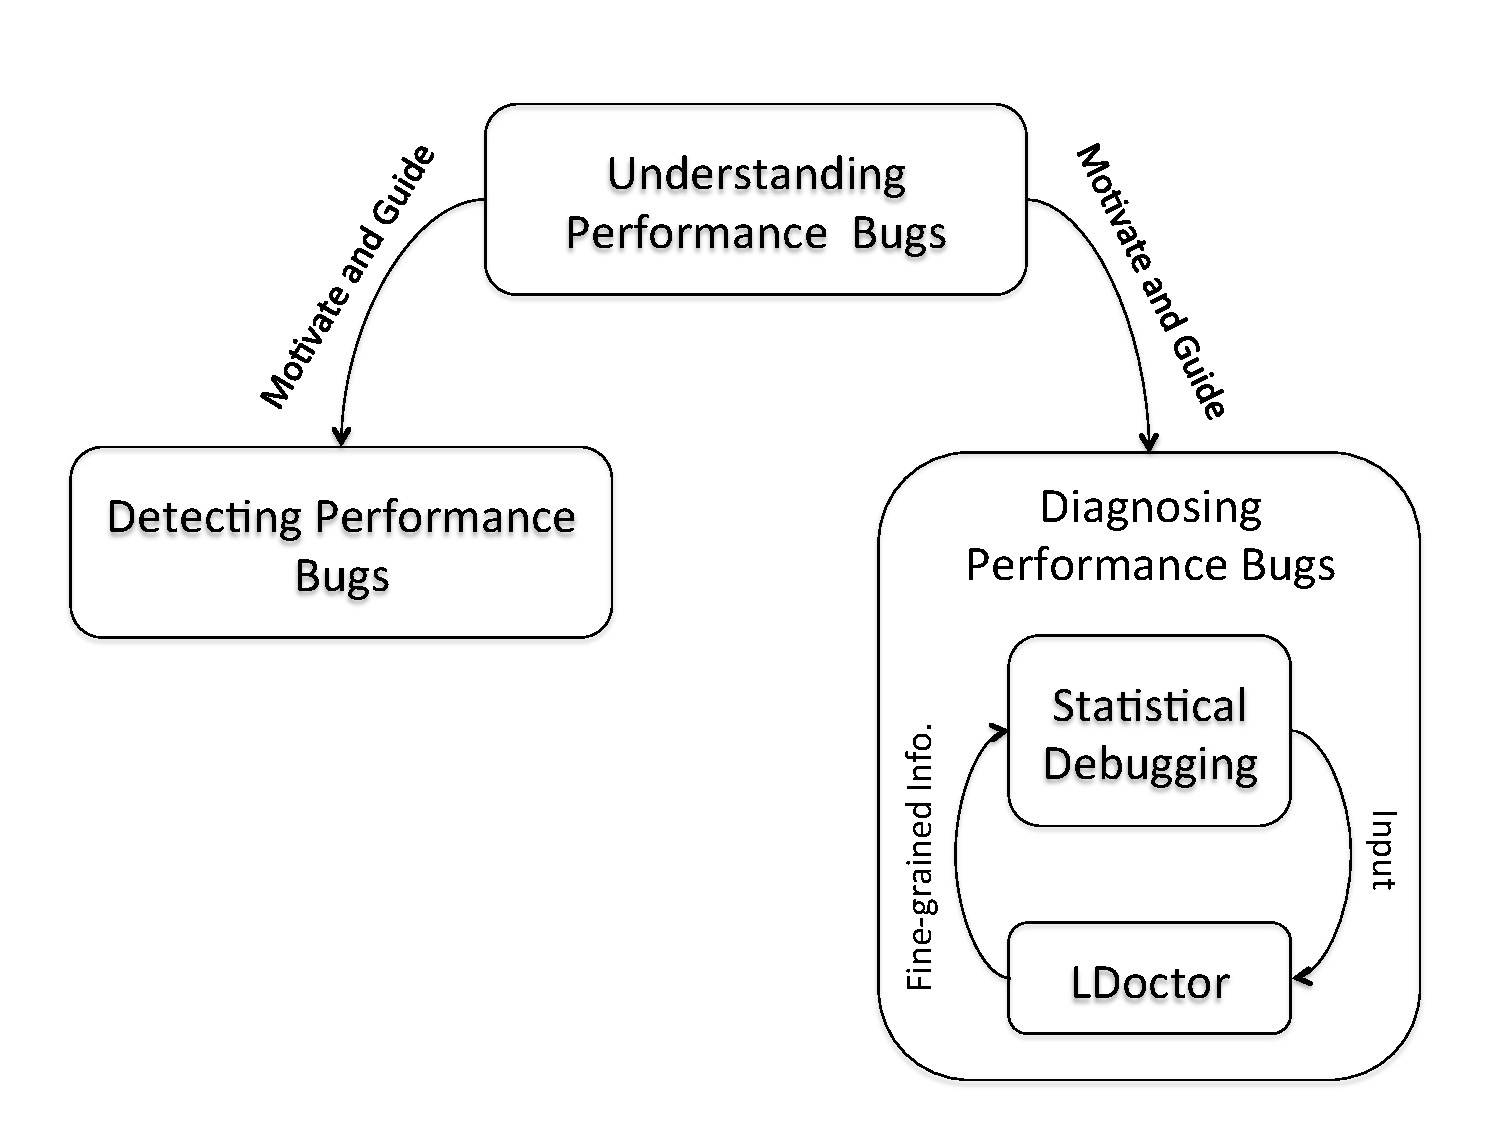
\includegraphics[width=4.5in]{figures/overview}
\caption{Interactions among the four components in this dissertation.}
\label{fig:overview}
\end{center}
\end{figure}

This dissertation works on three directions to address performance bug problems:
real-world performance bug understanding, 
performance bug detection and performance failure diagnosis. 
Specifically, we conduct the first empirical studies on real-world performance bugs. 
We examine final patches of fixed performance bugs, extract rules from these patches, 
and build checkers to detect violations to these rules. 
We explore the design space to apply statistical debugging to performance failure diagnosis. 
We build LDoctor, which is a brand new technique for inefficient loops, 
and can provide fine-grained diagnosis information.
These components of this dissertation interact and complement each other as shown in Figure~\ref{fig:overview}.

The dissertation work reflects the philosophy from three aspects. 
Firstly, empirical studies on functional bugs have already guided research in that area. 
The findings of our empirical study on performance bugs have also guided our own performance bug detection and diagnosis project. 
Secondly, rule-based bug detection has been widely used to detect functional bugs and security vulnerabilities. 
Our experimental results show that rule-based bug detection is also promising for performance bugs. 
Finally, statistical debugging is one of the most effective diagnosis techniques designed for functional bugs. 
Our evaluation shows that after choosing correct design points, statistical debugging can effectively diagnose performance bugs. 
Of course, performance bugs have their unique features, 
so LDoctor is designed solely for performance bugs. 

\subsection{Understanding performance bugs}

Addressing performance bug problems require approaches from different aspects, 
and all these aspects will benefit from a better understanding of performance bugs. 

This dissertation conducts a comprehensive characteristics study on 
a large number of real-world performance bugs collected from five widely used large open-source applications: 
Apache, Chrome, GCC, Mozilla and MySQL. 
This study reveals many interesting findings about performance bugs' root-cause patterns, 
how performance bugs are introduced, performance bugs' manifestation conditions, and fix strategies. 
It also directly motivates the following work on detecting and diagnosing performance bugs

\subsection{Rule-based performance bug detection}

Guided by our characteristics study, we hypothesize that 
(1) efficiency-related rules exist; 
(2) we can extract rules from performance-bug patches; 
and (3) we can use the extracted rules to discover previously unknown performance bugs. 
To test these hypotheses, we collect rules from 25 Apache, Mozilla, and MySQL bug patches 
and build static checkers to find violations to these rules.

Our checkers find 332 previously unknown Potential Performance Problems (PPPs) 
in the latest Apache, Mozilla, and MySQL. 
These include 219 PPPs found by checking an application using rules extracted from a different application. 
Our thorough code reviews and unit testings confirm that each PPP runs significantly slower 
than its functionality-preserving alternate suggested by the checker. 
We report some of found PPPs to developers. 77 PPPs are already confirmed by developers and 15 PPPs are fixed.  

The main contribution of our bug-detection work is that it 
confirms the existence and value of efficiency rules: 
efficiency rules in our study are usually violated at more than one place, 
by more than one developer, 
and sometimes in more than one program. 
Rule-based performance bug detection is a promising direction. 

\subsection{Statistical debugging for real-world performance bugs}
Statistical debugging is one of the most effective failure diagnosis techniques proposed for functional bugs. 
We explore how to apply statistical debugging to performance bugs. 

We first conduct an empirical study to understand how performance problems are observed and reported by real-world users. 
Our study shows that statistical debugging is a natural fit for diagnosing performance bugs, 
which are often observed through comparison-based approaches and reported together with both good and bad inputs. 
We then thoroughly investigate different design points in statistical debugging, 
including three different predicates and two different types of statistical models, 
to understand which design point works the best for performance diagnosis. 
Finally, we study how some unique nature of performance bugs allows sampling techniques 
to lower the overhead of run-time performance diagnosis without extending the diagnosis latency. 

\subsection{Performance diagnosis for inefficient loops}
Statistical debugging can accurately identify control-flow constructs 
that are most correlated with the performance problem by comparing problematic runs and regular runs. 
Unfortunately, for loop-related performance bugs, which contribute to
two thirds of real-world user-perceived performance bugs in our study, 
statistical debugging is not very effective.
Although statistical debugging can identify the root-cause loop, it does
not provide any information regarding why the loop is inefficient 
and hence is not very helpful in fixing the performance bug.

We build LDoctor, which is a series of static-dynamic hybrid analysis, for inefficient loops. 
We build LDoctor through two steps. 
The first step is to figure out a taxonomy of the root causes for common inefficient loops. 
The second step is to follow the taxonomy and design analysis for each root-cause subcategory. 
In order to balance accuracy and performance, we hybridize static and dynamic analysis. 
We further use sampling to lower the run-time overhead. 
Evaluation using real-world performance bugs show that LDoctor can provide good coverage and accuracy, 
with small run-time overhead.

\section{Dissertation Outline}
The remainder of this dissertation is organized as follows. 
\Cref{chap:background} describes the background knowledge and previous work on performance bug characteristics study, performance bug detection, performance failure diagnosis, and other related topics. 
\Cref{chap:study} presents our characteristics study of real-world performance bugs. 
\Cref{chap:detec} focus on our rule-based performance bug detection work. 
\Cref{chap:sd} explains our work to explore how to apply statistical debugging to performance failure diagnosis. 
\Cref{chap:ldoctor} presents LDoctor which can effectively diagnose inefficient loops. 
